\subsection{Procena radne sposobnosti}

Osoba, koja mo\v ze biti zaposlena ili ne, dolazi u Nacionalnu slu\v zbu za zapo\v sljavanje kako bi podnela zahtev za procenu radne sposobnosti nakon \v cega se formira komisija i vr\v si sam \v cin procene.

\begin{figure}[H]
	\centering
	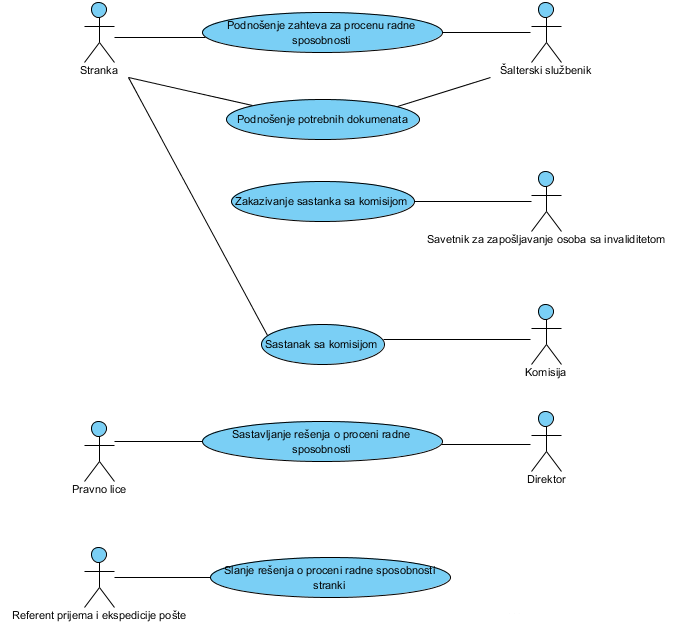
\includegraphics[width=\textwidth]{dijagrami/dijagrami-slucajeva-upotrebe/procena-radne-sposobnosti.png}
	\caption{Dijagram slu\v cajeva upotrebe procesa ''Procena radne sposobnosti''.}
	\label{dsu: procena_radne_sposobnosti}
\end{figure}


\subsubsection{Podno\v senje zahteva za procenu radne sposobnosti}

\noindent U\v cesnici: Stranka (S), \v Salterski slu\v zbenik (\v SS)
\\
\\ Preduslov: S se nalazi u sistemu Nacionalne slu\v zbe za zapo\v sljavanje i poneo je li\v cnu kartu.  \v SS je ulogovan na sistem.
\\
\\ Postuslov: S je uspe\v sno podnela zahtev.
\\
\\ Glavni tok:
\begin{enumerate}
	\item S prilazi automatu i bira opciju ''Zahtevi i molbe''.
	\item Automat bele\v zi da je opcija ''Zahtevi i molbe'' odabrana, ra\v cuna naredni broj u redu \v cekanja za tu opciju, i \v stampa papir sa brojem.
	\item S uzima broj i \v ceka svoj red.
	\item Kada do\dj e na red, S prilazi \v salteru i obave\v stava \v SS-a da \v zeli da podnese zahtev za procenu radne sposobnosti.
	\item \v SS tra\v zi li\v cnu kartu od S i ovaj mu je daje.
	\item \v SS pronalazi S u sistemu.
	\item \v SS predaje S-i da popuni zahtev za procenu radne sposobnosti.
	\item S popunjava zahtev nakon \v cega ga vra\' ca \v SS-u.
	\item \v SS proverava da li je sve ispravno popunjeno.
	\begin{enumerate}
		\item Ukoliko S nije ispravno popunio zahtev, \v SS mu vra\' ca da ispravi i dopuni zahtev. Prelazi se na korak 8 Glavnog toka.
		\item Ukoliko je S sve ispravno napisao prelazi se na korak 10 Glavnog toka.
	\end{enumerate}
	
	\item \v SS bele\v zi u sistem da je S podneo zahtev.
	\item \v SS \v salje S-i na e-mail adresu listu potrebnih dokumenata koje treba da donese i primer uplatnice radi pla\' cana tro\v skova procene radne sposobnosti.
	\item \v SS vra\' ca li\v cnu kartu S-i.
	\item Prelazi se na slu\v caj upotrebe \ref{su: podnosenje dokumenata}.
\end{enumerate}

\noindent Alternativni tok: /


\subsubsection{Podno\v senje potrebnih dokumenata}

\label{su: podnosenje dokumenata}

\noindent U\v cesnici: Stranka(S), \v Salterski slu\v zbenik (\v SS)
\\
\\ Preduslovi: \v SS je ulogovan na sistem.
\\
\\ Postuslovi: Dokumenta su porsle\dj ena Savetniku za zapo\v sljavanje osoba sa invaliditetom.
\\
\\ Glavni tok:
\begin{enumerate}
	\item S prilazi automatu i bira opciju ''Zahtevi i molbe''.
	\item Automat bele\v zi da je opcija ''Zahtevi i molbe'' odabrana, ra\v cuna naredni broj u redu \v cekanja za tu opciju, i \v stampa papir sa brojem.
	\item S uzima broj i \v ceka svoj red.
	\item Kada do\dj e na red, S prilazi \v salteru i saop\v stava \v SS-u da je sakupio potrebnu dokumentaciju.
	\item \v SS tra\v zi li\v cnu kartu od S i ovaj mu je daje.
	\item \v SS pronalazi S u sistemu.
	\item \v SS zatim tra\v zi dokumenta i uplatnicu od S i ovaj mu predaje.
	\item \v SS pronalazi S-u u sistemu.
	\item \v SS daje S-i da popuni upitnik.
	\item S popunjava upitnik i vra\' ca ga \v SS-u.
	\item \v SS proverava dokumenta i dokaz o uplati.
	\item \v SS pakuje sva dokumenta i upitnik u jednu fasciklu i prosle\dj uje je Savetniku za zapo\v sljavanje osoba sa invaliditetom.
	\item \v SS unosi u sistem da je S podneo potrebna dokumenta.
	\item \v SS vra\' ca li\v nu kartu.
	\item Prelazi se na slu\v caj upotrebe \ref{su: zakazivanje sastanka}
\end{enumerate}

\noindent Alternativni tok:
\begin{description}
	\item[A1. Fali neki dokument] ~\\
	Ukoliko u koraku 8 Glavnog toka \v SS ustanovi da S nije doneo sva potrebna dokumenta ili dokaz o uplati, \v SS mu govori koja dokumenta mu fale. Slu\v caj upotrebe se ovde zavr\v sava.
\end{description}

\subsubsection{Zakazivanje sastanka sa komisijom}

\label{su: zakazivanje sastanka}

\noindent U\v cesnici: Savetnik za zapo\v sljavanje osoba sa invaliditetom (SZ)
\\
\\ Preduslov: SZ ima potrebnu dokumentaciju.
\\
\\ Postuslov: Zakazan je sastanak sa komisijom.
\\
\\ Glavni tok:
\begin{enumerate}
	\item SZ pronalazi stranku u sistemu.
	\item SZ uzima dokumentaciju i skenira je.
	\item SZ \v salje e-mail radniku u PIO da je potrebno sastaviti komisiju za procenu radne sposobnosti i u njemu skeniranu dokumentaciju.
	\item Kada radnik u PIO odgovori sa podacima o komisiji i terminu sastanka, SZ \v salje podatke o sastanku stranki na e-mail.
	\item SZ unosi podatke o sastanku i komisiji u sistem.
	\item SZ priprema dokumentaciju za komisiju i prosle\dj uje je.
	\item Prelazi se na slu\v caj upotrebe \ref{su: sastanak}.
\end{enumerate}

\noindent Alternativni tok: /


\subsubsection{Sastanak sa komisijom}

\label{su: sastanak}

\noindent U\v cesnici: Komisija (K), Stranka (S)
\\
\\ Preduslovi: K ima potrebnu dokumentaciju.
\\
\\ Postuslovi: K je analizirala slu\v caj i sastavila nalaz.
\\
\\ Glavni tok:
\begin{enumerate}
	\item S dolazi u dogovorenu prostoriju u zakazano vreme.
	\item K vr\v si pregled S-e.
	\item K analizira dokumentaciju.
	\item K saop\v stava S-i da je sastanak zavr\v sen i da \' ce po\v stom biti obave\v sten o odluci.
	\item S odlazi.
	\item K sastavlja nalaz.
	\item K prosle\dj uje nalaz Pravnom licu.
	\item Prelazi se na slu\v caj upotrebe \ref{su: resenje o rs} 
\end{enumerate}

\noindent Alternativni tok: /


\subsubsection{Sastavljanje re\v senja o proceni radne sposobnosti}
\label{su: resenje o rs}
\noindent U\v cesnici: Pravno lice (PL), Direkotor (D)
\\
\\ Preduslovi: PL je dobio nalaz komisije.
\\
\\ Postuslovi: PL je sastavio re\v senje i D ga je potpisao.
\\
\\ Glavni tok:
\begin{enumerate}
	\item PL analizira nalaz.
	\item PL tuma\v ci zakon.
	\item PL na osnovu zakona i nalaza sastavlja re\v senje.
	\item PL odnosi D-u da potpi\v se re\v senje.
	\item D \v cita i potpisuje re\v senje.
	\item PL overava re\v senje i prosle\dj uje ga pisarnici. 
	\item Prelazi se na slu\v caj upotrebe \ref{su: slanje resenja o radnoj sposobnosti}
\end{enumerate}

\subsubsection{Slanje re\v senja o proceni radne sposobnosti stranki}
\label{su: slanje resenja o radnoj sposobnosti}

\noindent U\v cesnici: Referent prijema i ekspedicije po\v ste (RPEP).
\\
\\ Preduslovi: PL je prosledio overeno re\v senje u pisarnicu.
\\
\\ Postuslovi: Rešenje o proceni radne sposobnosti je poslato stranki.
\\
\\ Glavni tok:
\begin{enumerate}
	\item RPEP preuzima overeno re\v senje o proceni radne sposobnosti.
	\item RPEP pakuje re\v senje u kovertu.
	\item RPEP \v cita adresu stranke iz sistema.
	\item RPEP \v salje overeno re\v senje na pro\v citanu adresu.
\end{enumerate}


\noindent Alternativni tok: /

\begin{mylandscape}
	\subsubsection{BPMN dijagrami}
	
	\begin{figure}[H]
		\centering
		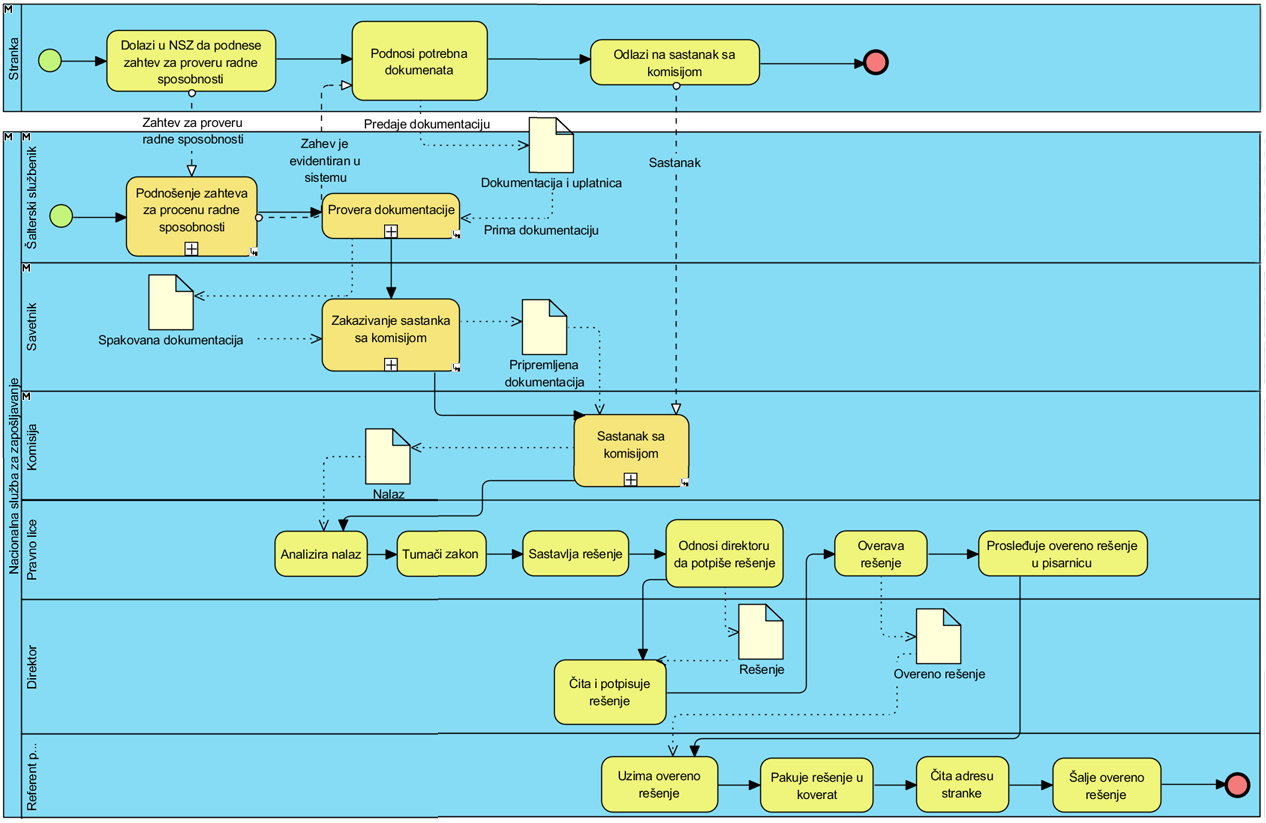
\includegraphics[width=0.8\paperwidth]{dijagrami/bpmn-dijagrami/procena-radne-sposobnosti.png}
		\caption{BPMN dijagram procesa ''Procena radne sposobnosti''.}
		\label{bpmnd: procena radne sposobnosti}
	\end{figure}
	
	\newpage
	
	\begin{figure}[H]
		\centering
		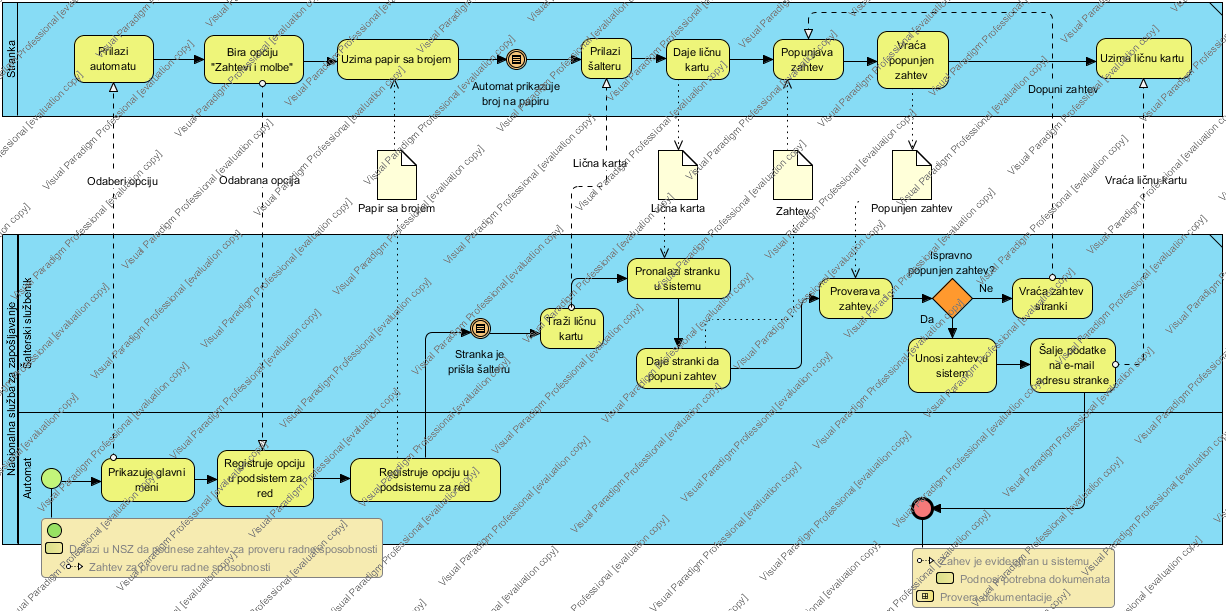
\includegraphics[width=0.8\paperwidth]{dijagrami/bpmn-dijagrami/podnosenje-zahteva-za-procenu-radne-sposobnosti.png}
		\caption{BPMN dijagram potprocesa ''Podno\v senje zahteva za procenu radne sposobnosti'' procesa ''Procena radne sposobnosti'' (Slika \ref{bpmnd: procena radne sposobnosti}).}
	\end{figure}
	
	\newpage
	
	\begin{figure}[H]
		\centering
		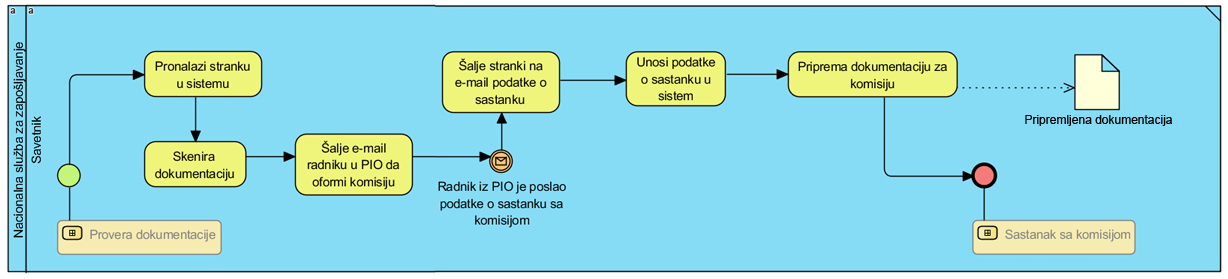
\includegraphics[width=0.8\paperwidth]{dijagrami/bpmn-dijagrami/zakazivanje-sastanka-sa-komisijom.png}
		\caption{BPMN dijagram potprocesa ''Zakazivanje sastanka sa komisijom'' procesa ''Procena radne sposobnosti''  (Slika \ref{bpmnd: procena radne sposobnosti}).}
	\end{figure}

	\newpage
	
	\begin{figure}[H]
		\centering
		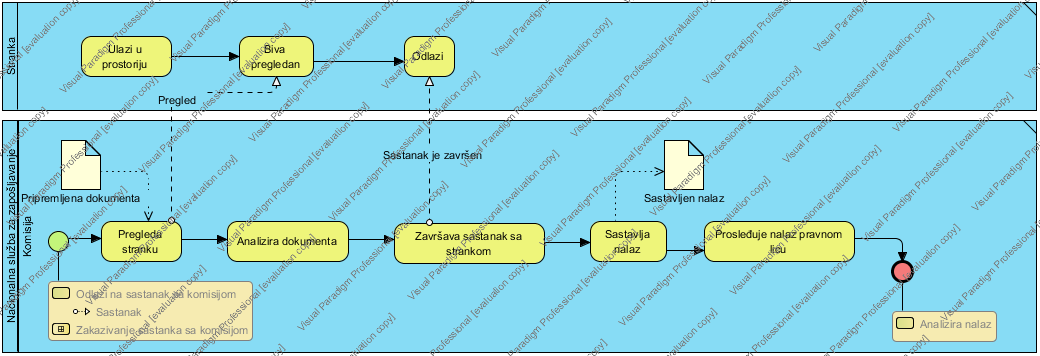
\includegraphics[width=0.8\paperwidth]{dijagrami/bpmn-dijagrami/sastanak-sa-komisijom.png}
		\caption{BPMN dijagram potprocesa ''Sastanak sa komisijom'' procesa ''Procena radne sposobnosti''  (Slika \ref{bpmnd: procena radne sposobnosti}).}
	\end{figure}
\end{mylandscape}

